% this file is called up by thesis.tex
% content in this file will be fed into the main document
\chapter{Knowledge-Based Design} % top level followed by section, subsection
%: ----------------------- paths to graphics ------------------------

% change according to folder and file names
\ifpdf
    \graphicspath{{3/figures/PNG/}{3ures/PDF/}{2.5/figures/}}
\else
    \graphicspath{{3/figures/EPS/}{3/figures/}}
\fi

%: ----------------------- contents from here

%\begin{flushright}
%An amazing thing, the human brain
%\linebreak
%apable of understanding incredibly complex
%\linebreak
%and intricate concepts. Yet at times unable
%\linebreak
%to recognize the obvious and simple.
%\linebreak
%Jay Abraham 
%\end{flushright}

\label{KBDchapter}
It is common for all companies to keep archives of previous successful designs. As a consequence, irrespective of the design method adopted, there are often reasons for new designs to be based on ``similar" previous ones, instead of starting the design procedure from scratch. As a matter of example, if for instance a new turbomachinery rotor is to be designed, a useful ``similar'' design might be a rotor successfully  designed in the past for ``slightly'' different operating conditions and/or ``slightly'' different objectives or constraints. 
In some cases, these designs might have been performed enough time ago, using ``old-fashioned'' design procedures according to different paremeterizations. In general, the term Knowledge-Based System (KBS) \cite{Akerkar:2009:KS:1795845} is used to describe methods and processes for designing new products, engines, services etc.\ based on stored/archived knowledge which is available in the form of previous successful designs.                

In this thesis, a new design method, to be referred to as  Knowledge-Based Design (KBD), which combines EAs with principles and concepts from Knowledge-Based Systems (KBS) in order to create an automated design procedure, is proposed. It employs a KBS similar to Case-Based Reasoning (CBR) \cite{kolodner_1991,kolodner_1993,slade_1991,riesbeck_1989}, in order to utilise/exploit the availability of an archive of successful designs. In the design of aero- or hydrodynamic shapes, a pattern of similar geometries often occurs when dealing with similar problems. For example, the optimal airfoil, regarding objective(s) ``A" and constraint(s) ``B", of a compressor cascade operating at conditions ``C" and inlet flow angle $\alpha_1$ (where ``C'' includes everything but $\alpha_1$) will be, more or less, similar to the airfoil of a different compressor designed for the same ``A", ``B" and ``C" and inlet flow angle equal to $\alpha_1\!+\!1^o$.  Therefore, if a design is optimal for a set of different/neighbouring conditions, it still holds valuable information about the design space that can be exploited in order to speed-up the design process. This is the main purpose of the proposed KBD method which shares the advantages of both EAs and KBS.    

In more detail, from the CBR point of view, the proposed methodology achieves in creating a fully automated and time-efficient \textit{revise} step, this is the step that adapts the existing ``similar" designs so as to make them perform optimally at the new operating conditions and/or according to the new objectives. In this thesis, this is achieved by using an EA as a revise tool. In order to have a cost-efficient procedure, capable for being routinely used in an industrial environment, additional EA speed-up techniques, mainly the use of metamodels (MAEA, section \ref{MAEApar}), are employed. The straightforward way to achieve this goal would be to simply inject the ``similar" archived designs into the initial population of an EA, by replacing some of the randomly generated population members.
In contrast, the method proposed in this thesis utilizes statistical analysis to introduce a new set of design variables, based on the archived designs, in order to further speed-up the EA itself. This is achieved through:  
%Regarding EAs the proposed method achieves three important goals: 
\begin{description}
  \item[a)]The significant reduction in problem dimension (i.e.\ the number of design variables handled by the EA), thus improving both the EA (faster convergence to the optimal solution) and MAEA efficiencies (use of ANNs as metamodels  with greater prediction accuracy and without delaying the start of the IPE phase, as described in section \ref{MAEApar}). 
  \item[b)]The automatic definition of the newly introduced design variables' (to be referred to as optimization variables, to distinguish them from the design variables used to parameterize the geometry) range; the designer overcomes the burden of arbitrarily guessing their lower and upper bounds and, therefore, eliminates the possibility of accidentally excluding search sub-areas corresponding to the optimal design. 
    \item[c)]The association of degrees of importance to the optimization space regions. Practically, higher probability to host candidate solutions is given to the regions of the design space pinpointed by the statistical analysis of the archived ``similar" designs, based on a pre-defined probability distribution. This allows the exploration of extended design spaces, with different levels of importance associated with different sub-regions, according to statistics.
\end{description}

%All the above allow the exploitation of extended design spaces, both in number of design variables and effective range for each one of them, in an efficient way by exploiting the information incorporated in archived "similar" designs.     

\section{Knowledge-Based Systems (KBS)}  
KBS \cite{Akerkar:2009:KS:1795845}  are systems based on methods and techniques of artificial intelligence. Their core components are the knowledge base and inference mechanisms. In this thesis, a KBS named Case-Based Reasoning (CBR) \cite{kolodner_1991} is combined with EAs, in an optimal way, giving rise to the KBD method. For reasons of clarity, a brief introduction to the CBR method follows, before presenting the proposed KBD method.  

%***********************************************************************
\subsection{Case-Based Reasoning Method - Principles}
%***********************************************************************
CBR, \cite{kolodner_1991,kolodner_1993,slade_1991,riesbeck_1989}, can be seen as a problem solving method that reuses past cases and experience to conceive a solution to the current problem, 
whereas other major artificial intelligence techniques rely on mapping generalized 
relationships between problem descriptions and conclusions. CBR has the advantage 
of utilizing  experience based on past successful problem solutions. 
The main tasks of a CBR system is to identify the problem in hand, find one or 
more similar past case(s), use this information to suggest a solution to the current 
problem and update the system by learning from this experience.      

\label{History} The origins of CBR dates back to the work by
Schank and Abelson in 1977, \cite{Schank_Abelson_1977}. They proposed that general 
human knowledge about situations is recorded as scripts that allow extracting 
 expectations and inferences. Scripts were proposed as structures for conceptual 
memory describing information about stereotypical events. However, experiments 
showed that this is not a complete theory of memory representation since people 
often confuse events with similar scripts. These conform with 
concept formulation, problem solving and experimental learning theories within 
philosophy and psychology, \cite{tulving_1977,smith_1978}. 

Schank continued to investigate the role of previous situations (i.e.\ cases) 
and situation patterns in both problem solving and learning, \cite{Schank_1982}.  
Simultaneously, Gentner, \cite{genter_1983}, developed a  
theoretical framework for analogy also relevant to CBR. Significant references to CBR can also be found in 
Wittgensteins observation, \cite{wittgestein_1953}, that natural concepts are in fact 
polymorphic and cannot be classified by a single set of necessary and sufficient 
features; instead they can be defined by a set of instances (i.e.\ cases) with family 
resemblances. The latter work has been cited as the philosophical basis for CBR by Aamondt and Plaza, \cite{aamond_plaza_1994}.

Though the roots of CBR could be claimed by several scientists, it was Schank and his co-workers who, in the early 80's, developed a cognitive model which the first CBR applications were based upon. Kolonder developed the first CBR system named CYRUS, \cite{kolodner_1983a,kolodner_1983b}, which was an implementation of Schank's dynamic memory model. Later, its case-memory model served as the basis for several other CBR systems and was used in various disciplines ranging from law, \cite{ashley_1988,rissland_skalak_1989}, to civil engineering, \cite{whatson_abdullah_1994,moore_1994}.

\label {CBR}  The classical definition of CBR was coined by Riesbeck and Schank, \cite{riesbeck_1989}: \textit{``A case-based reasoner solves problems by using or adapting solutions to old problems"}. This clearly defines what a CBR system can do, without however determining the way of doing it. This can be graphically understood by the so-called CBR-cycle (fig.\ \ref{cbr}).  The CBR-cycle is based on four logical steps, as defined by Aamodt and Plaza, \cite{aamond_plaza_1994}, which are often referred to as the four REs: 

\begin{itemize}
  \item RETRIEVE the most ``similar" case(s),
  \item REUSE the retrieved case(s) for the problem in hand,
  \item REVISE the case(s), if necessary, and
  \item RETAIN the new solution in the archive for future use.
\end{itemize}
The four REs can be represented by a schematic cycle, fig.\ \ref{cbr}.

In the proposed KBD method, the REVISE step is undertaken by an EA which automatically combines the RETRIEVED cases without requiring human intervention. Recall that the traditional CBR method requires a human expert to undertake task.  

%\figuremacroW{cbr}{Schematic cycle representing the CBR-cycle}{0.5}
\begin{figure}[h!]
\begin{minipage}[b]{1\linewidth}
 \centering
 \resizebox*{!}{10 cm}{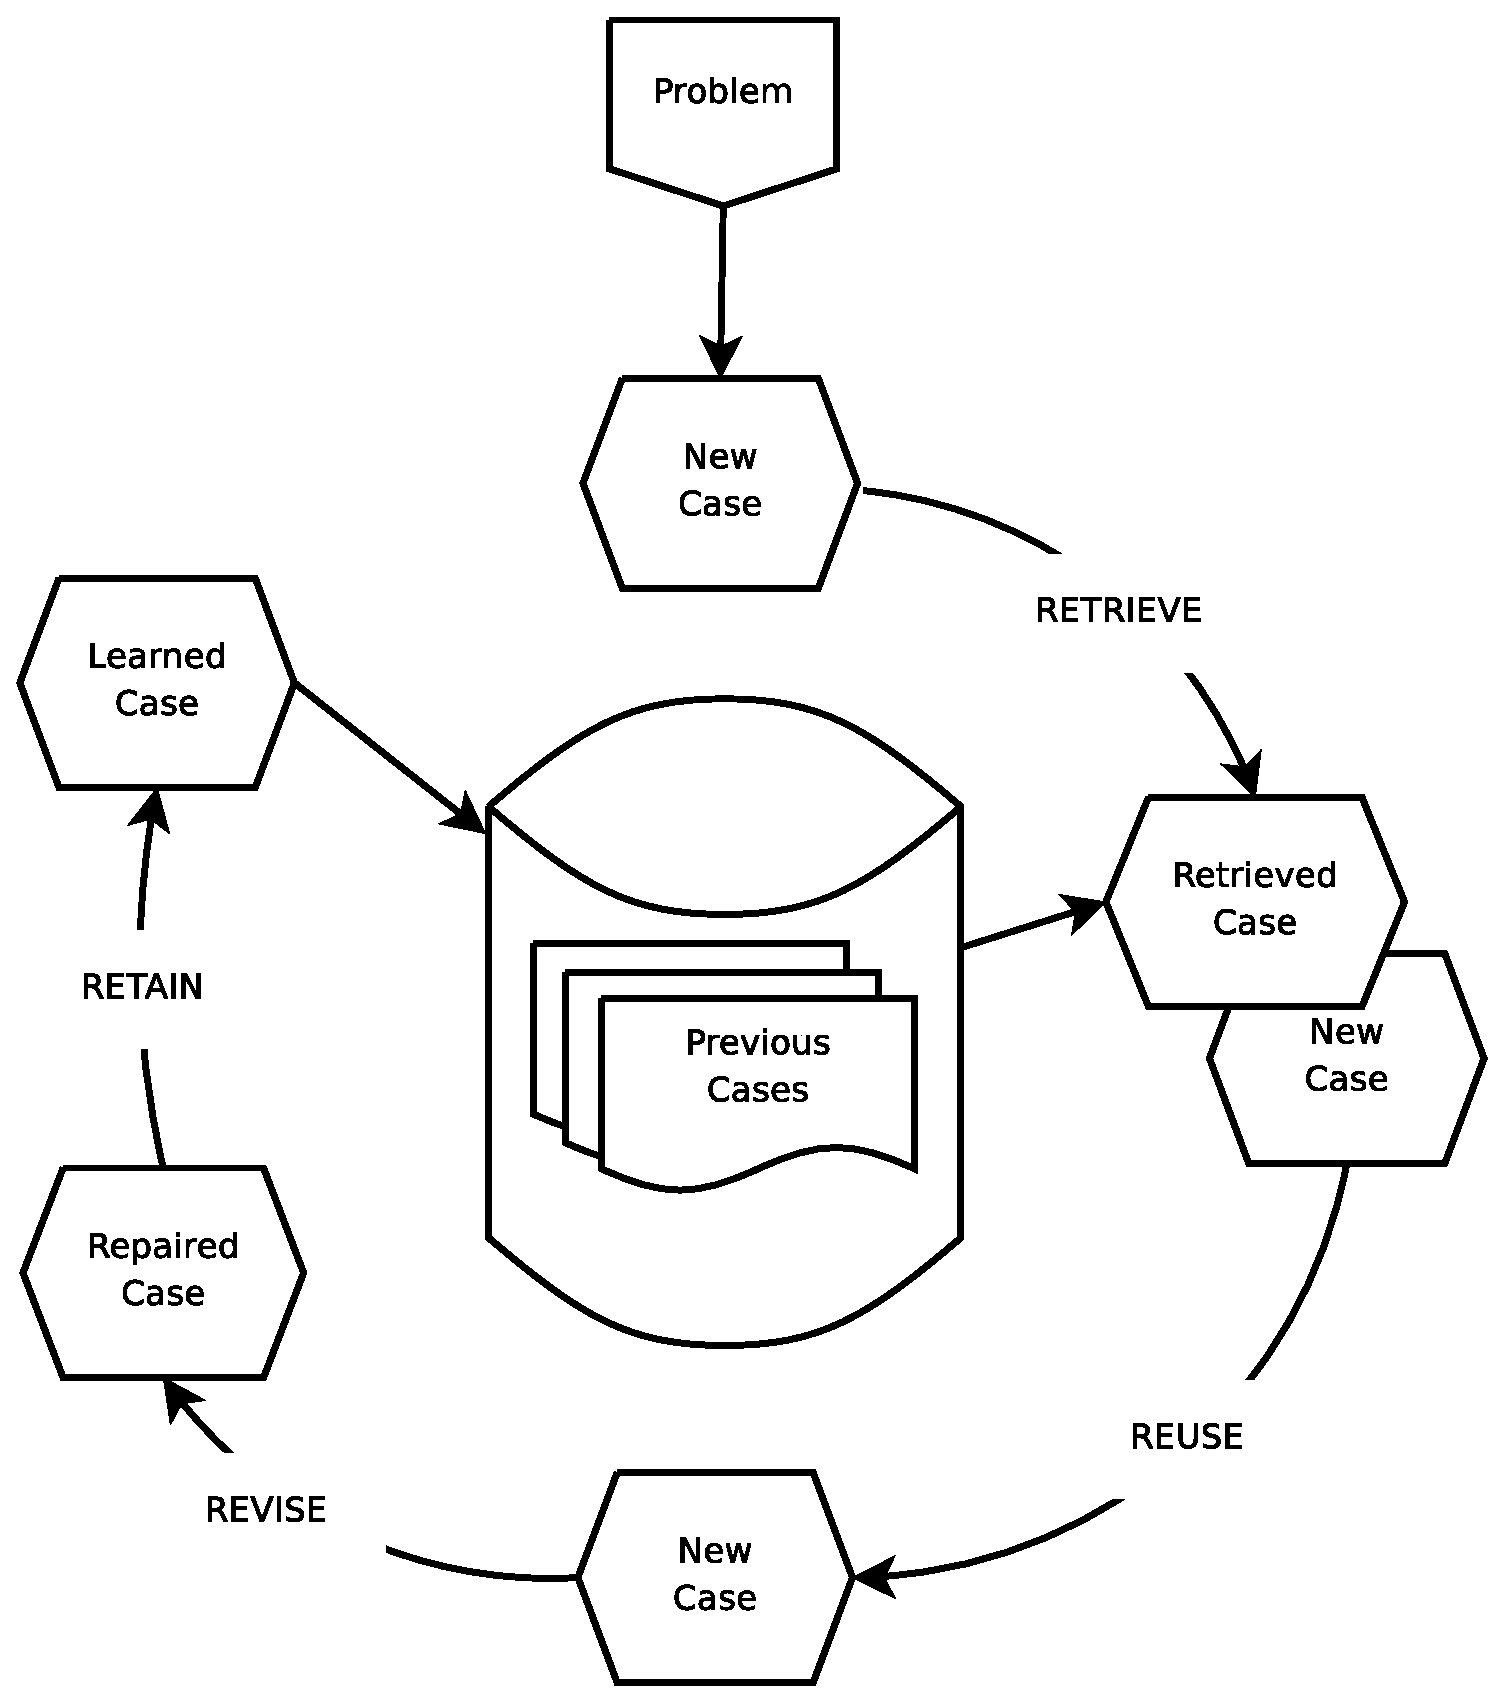
\includegraphics{cbr.eps}}
\end{minipage}
\caption{Schematic representation of the CBR-cycle; from \cite{aamond_plaza_1994}.} 
\label{cbr}
\end{figure}

%%%%%%%%%%%%%%%%%%%%%%%%%%%%%%%%%%%%%%%%%%%%%%%%%%%%%%%%%%%%%%%%%%%%%%%

\section{The KBD Method}

%In case of shape design problems in fluid mechanics with specific characteristics in a specific environment, due to the nature of the problem, the solution is always complex. Thus the need of adaptation (revise) is almost certain. \textit{Null adaptation is useful for problems involving complex reasoning but with a simple solution.}

In order to have a fully automated REVISE step, a set of adaptation rules must replace human intervention. These rules take into account the deviations of the proposed solution from the desired one and suggest an improved proposal. The rules governing the evolution of species ideally fit the above description. So, in this thesis, an EA is proposed to undertake the REVISE step. 

Therefore, the present method aims at extending the optimization method by making it capable to accommodate and exploit pieces of useful information archived during previous relevant successful designs. The KBD method is much more elaborated than the simple and straightforward injection of retrieved designs in the initial population of an EA, where they replace some of the randomly generated ones. Instead, the KBD method  introduces a new set of unknowns, the so-called optimization variables, to be used by the EA, instead of the design variables. In case of complex 3D geometries, such as those involved in the field of thermal and hydraulic turbomachines, the number of design variables is much greater and this slows the design-optimization process down. The optimization variables are introduced by expressing the candidate solutions as points in the optimization space, which is the space defined by the design vectors of the retrieved geometries as vector bases. The role of the optimization algorithm is to find the value set (or sets, for more than one objectives, in problems where the Pareto front of non-dominated solutions is sought) of the optimization variables which yields optimal performance. Since the number of optimization variables is much less than the number of design variables, the number of degrees of freedom is reduced and the EA or MAEA CPU cost is expected to be much lower.

\subsection{Optimization Variables's Definition}
In this section, the optimization variables introduced by the proposed KBD method are presented. Assume that a small number (m) of previous designs are retrieved from the archive. These designs must correspond to similar problems, as already discussed. For the proposed method, it is necessary  for the retrieved geometries to be expressed in terms of the same parameterization. If techniques able to transform a parameterization scheme to any other (within a degree of accuracy, of course) are available, this task is straightforward. Let us denote by $GEO_i=(x_1^i,x_2^i,....,x_N^i)$, $i\!=\!1,m$ the m archived designs, with $N$ design variables each.

The set of optimization variables can be defined, without yet associating any degree of importance to the optimization space subregions, by assuming that each new design $x_j^{new}$ results from the combination of the $m$ archived designs, weighted by the  $w_i$ $(i=1,m)$, or

\begin{eqnarray}
   x_j^{new} = \frac{\sum_{i=1}^{m}w_i x_j^i}{\sum_{i=1}^{m}w_i },~~~ j=1,...,N 
   \label{linear} 
\end{eqnarray}
Without loss in generality, one may assume that $w_i \in [0,1]$. 

Next step is the association of degrees of importance to the optimization space regions. This is achieved by rewriting eq. \ref{linear} as

\begin{eqnarray}
   x_j^{new} = \Phi _j^{-1} (\frac{\sum_{i=1}^{m}w_i \Phi _j(x_j^i)}{\sum_{i=1}^{m}w_i }) 
   \label{non-linear} 
\end{eqnarray}
through the introduction of the sigmoid cumulative distribution function $\Phi$,  \cite{Kiemele}, according to a user-defined probability distribution function. If the normal distribution function is used, $\Phi$ is given by

\begin{eqnarray}
   \Phi _{\mu \sigma ^2} (x)= \frac{1}{\sigma\sqrt[2]{2\pi}}\int _{-\infty}^x exp(\frac{-(u-\mu)^2}{2 \sigma^2}) 
   \label{cdf} 
\end{eqnarray}
where $\mu$ is the mean value and $\sigma$ the standard deviation of each design variable (j). Schematically,
\begin{eqnarray}
		\left( {\begin{array}{c}
 		x_1^1  \\
 		\vdots  \\
 		x_N^1	\\
 		\end{array} } \right) 
 		\left( {\begin{array}{c}
 		x_1^i  \\
 		\vdots  \\
 		x_N^i	\\
 		\end{array} } \right)
 		\left( {\begin{array}{c}
 		x_1^m  \\
 		\vdots  \\
 		x_N^m	\\
 		\end{array} } \right) \rightarrow
		\left( {\begin{array}{c}
 		\mu _1  \\
 		\vdots  \\
 		\mu _N  \\
 		\end{array} } \right)
		\left( {\begin{array}{c}
 		\sigma _1  \\
 		\vdots  \\
 		\sigma _N  \\
 		\end{array} } \right)
   \label{cdf-matrix} 
\end{eqnarray}


 
%Among other, the set of the archived solutions reveals the statistical distribution of each design variable and, consequently, this can be used both to introduce importance to the design space regions and also set the bounds of the design space. This is achieved by, instead of eq. \ref{linear}, the nonlinear equations

%
%are to be used in order to define the new optimization variables. In eq. \ref{non-linear}, $\Phi _j$ are appropriate nonlinear functions. Based on the assumption that the retrieved designs correspond to operating conditions correlated to the new ones, the new design should conform to a normal distribution. Should this be the case, the sigmoid cumulative distribution function could be used for $\Phi _j$  \cite{Kiemele}. 

Since the m retrieved designs are usually located ``around'' the desired one in the operating conditions space and based on the assumption that this information is, more or less, transferable to the design space, the  normal probability distribution is used to assign degrees of importance throughout this thesis. In a simplified example, the above statement says that: Assume that airfoil A with design variables vector $\vec{x}_A$ is optimal, regarding objective(s) ``O'', when operating at conditions ``C''. Assume, also, that at these conditions the flow turning is equal to $\Delta a\!=\!40^o$. Also,  that design B, or $\vec{x}_B$,  is optimal regarding the same objectives at the same conditions and delivers flow turning equal to $\Delta a \!=\!41^o$. Considering the same objectives ``O'' and the same conditions ``C'', if the optimal airfoil which delivers flow turning equal to $\Delta a\!=\!40.5^o$ is sought, the optimal design N, or $\vec{x}_N$, would, most probably, be close to  $\frac{\vec{x}_A+\vec{x}_B}{2}$ which is the vector of the mean values of the design variables of the retrieved geometries A and B. It is reminded that, if the normal probability distribution is used for importance assignment, the regions near the mean value of each design variables will be assigned the highest importance and, therefore, highest probability to accommodate candidate solutions. In case the user knows in advance that, for this particular problem, the above statement is not true, he might exchange the normal distribution with the appropriate probability distribution of his choice.           

The use of the cumulative distribution function of the normal probability distribution, eq.\ \ref{cdf}, practically assumes the bounds of $b_i$ to be within $\mu _i \pm 3\sigma _i$, \cite{Kiemele}. To overcome this limitation, a single extrapolation variable $\Psi$ which multiplies all $\sigma$ values computed based on the archived designs and extends the search space outside $\mu _i \pm 3\sigma _i$, is optionally introduced. $\Psi$ is multiplied with the computed standard deviations to yield the ones used in eq.\ \ref{cdf}, as follows


\begin{eqnarray}
		\left( {\begin{array}{c}
 		\sigma _1  \\
 		\vdots  \\
 		\sigma _n  \\
 		\end{array} } \right) =
 		\Psi  
 		\left( {\begin{array}{c}
 		\sigma _1^{computed}  \\
 		\vdots  \\
 		\sigma _n^{computed}  \\
 		\end{array} } \right)
   \label{cdf-matrix} 
\end{eqnarray}


If the available archived designs are not that many, which often is the case, then $m$ is a significantly small integer.  With either eq.\ \ref{linear} or \ref{non-linear}, an optimization problem with only $m$ weights as unknowns may loose its flexibility. Such a method may overcome the curse of dimensionality (since the number of optimization variables is  noticeably lower than $N$) but may lead to sub-optimal solutions. To overcome this, the grouping of those design variables which are ``co-related''. Relevant design variables such as, for instance, those defining the mean camber surface angle at the leading edge etc.\ are grouped together. After forming these groups, a different weight is associated with each one of them. The new weights are denoted by $w_{i,k}$, where the first index corresponds to the $i^{th}$ design basis and the second one to the $k^{th}$ group of design variables (where $b_i$ belongs to). Finally, instead of either eq.\ \ref{linear} or \ref{non-linear}, the expression


\begin{eqnarray}
   x_j^{new} = \Phi _j^{-1} (\frac{\sum_{i=1}^{m}w_{i,k} \Phi _j(x_j^i)}{\sum_{i=1}^{m}w_{i,k} }),~ k=f(j) 
   \label{non-linear2} 
\end{eqnarray}
can be used. 

Based on eq.\ \ref{non-linear2}, an optimization problem with $m  K$ unknowns (or $m K\!+\!1$, to also account for $\Psi$), where $K$ is the number of design variable groups, is formulated. Population-based search methods, such as EAs (or MAEAs), with the proposed parameterization, may locate the global optimum much more efficiently than an EA (or MAEA) based on the conventional parameterization. This is demonstrated on the solution of  thermal (section \ref{Drela1}) and hydraulic (section \ref{Francis-runners}) turbomachinery design-optimization problems. 


%\begin{figure}[h!]
%\begin{minipage}[b]{0.9\linewidth}
% \centering
% \resizebox*{9cm}{!}{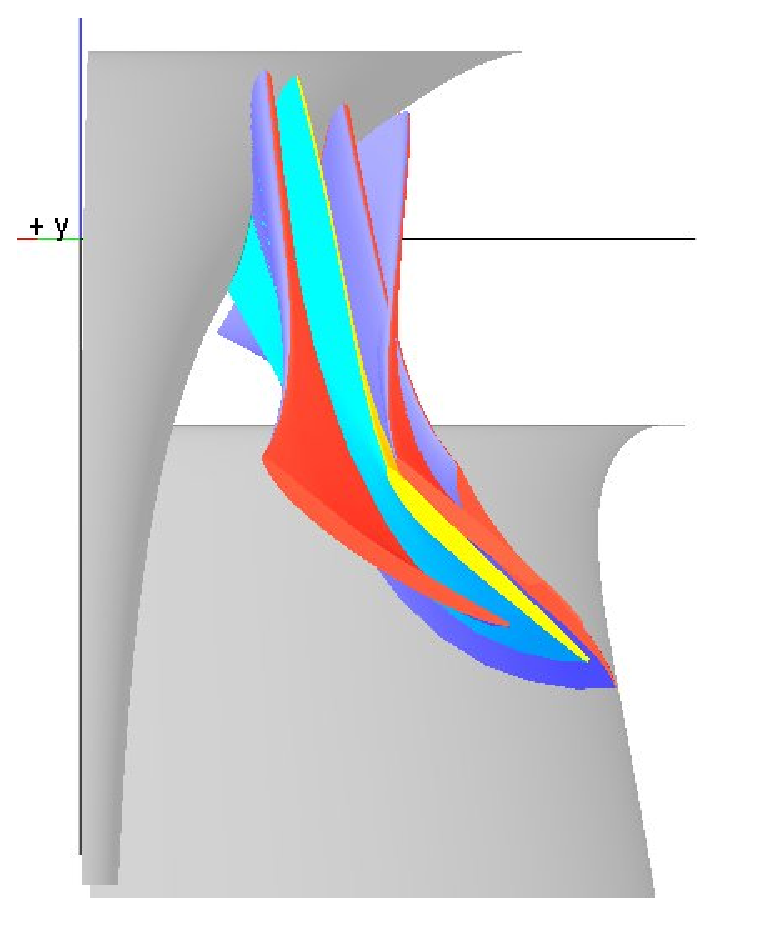
\includegraphics{cbr_r.eps}}
%\end{minipage}
%\caption{A new Francis blade (section \ref{Francis-runner}) (\ifcolore light blue and yellow\else light gray\fi) is designed on the basis of 3 %archived designs (\ifcolore dark blue and red\else dark gray\fi).} 
%\label{CBRtemp1}
%\end{figure}


%\begin{figure}[h!]
%\begin{minipage}[b]{0.9\linewidth}
% \centering
% \resizebox*{12cm}{!}{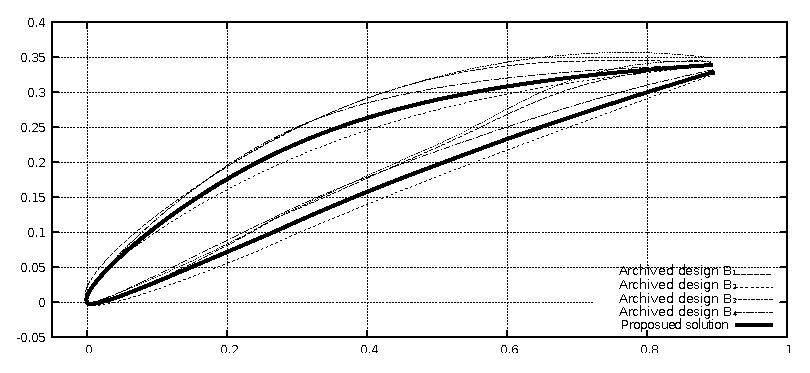
\includegraphics{blade.eps}}
%\end{minipage}
%\caption{A new airfoil (continuous line) is designed on the basisof 4 archived designs (dotted lines).} 
%\label{CBRtemp2}
%\end{figure}

%Two applications of the KBD method, for the design of a Francis hydraulic turbine and a compressor cascade, are presented in fig.\ref{CBRtemp1} and fig.\ref{CBRtemp2} respectively. The Francis blade (fig.\ref{CBRtemp1}) is generated from the KBD method using three archived designs (\ifcolore dark blue designs\else dark gray\fi). Using the KBD method a significant  reduction in the design parameters was achieved, from $336$ to $19$  ($3$ bases $\times 6$ groups $+1$ extrapolation parameter) (for more information see section \ref{Francis-runner}). The compressor cascade (fig.\ref{CBRtemp2}) is design using four archived designs (dotted lines) and the number of design parameters was decreased from 27 to 13 ($4$ bases $\times 3$ groups $+1$ extrapolation parameter).

\section{Design of a Compressor Cascade using KBD}
\label{Drela1}
The design of a 2D compressor cascade operating at $M_1\!=\!0.54$, $a_1\!=\!44^o$ and $Re\!=\!4\times10^5$ (Reynolds number based on the chord) for minimum total pressure losses is sought. Losses are measured in terms of the total pressure loss coefficient 
\begin{eqnarray}
   \omega=\frac{p_{t1}-p_{t2}}{p_{t1}-p_1}
   \label{omegaLosses} 
\end{eqnarray}
where indices $1$ and $2$ denote the cascade inlet and outlet, respectively. 
The blade airfoil is designed subject to a number of aerodynamic and geometrical constraints: the optimal airfoil must turn the flow by more than $30^o$ and its thickness at three chordwise positions ($0.3c$, $0.6c$ and $0.9c$) must be greater than $0.10c$, $0.08c$ and $0.01c$,  respectively.     

The airfoil shape is parameterized based on the mean-camber line shape and thickness distributions (separately for the pressure and  suction sides). All of them are parameterized using NURBS. The mean-camber line parameterization ``introduces'' three degrees of freedom, namely the leading edge (LE) angle, the trailing edge (TE) angle and the weight associated with the second control point. The suction side thickness distribution is controlled by $9$ design variables, namely the $x$ and $y$ coordinates as well as the weights of three, out of the five, internal NURBS control points. The first and last control points are fixed at the predefined LE and TE positions. The pressure side thickness distribution is controlled via 15 design variables, standing for the $x$ and $y$ coordinates as well as the weights of five, out of the eight, internal control points. The first and last control points are fixed at the predefined LE and TE positions and the location of the second point is determined by the requirement of first-order continuity at the LE.  The total number of design variables describing each candidate solution is $27$, fig.\ \ref{CBRparam}. 

\begin{figure}[h!]
\begin{minipage}[b]{1\linewidth}
 \centering
 \resizebox*{15cm}{!}{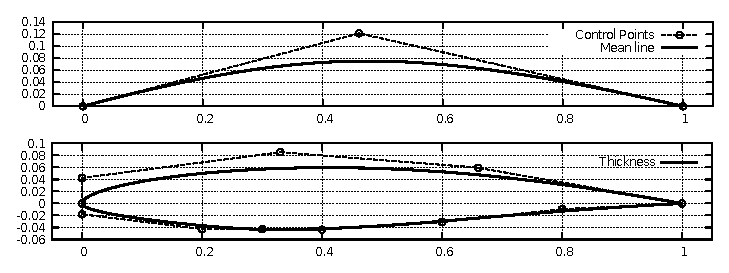
\includegraphics{airf.eps}}
\end{minipage}
\caption{Design of a compressor cascade using KBD: Top: parameterization of the mean-camber line with $3$ control points. Bottom:  parameterization of the thickness distributions with NURBS using $5$ control points for the suction side and $8$ for the pressure side. The total number of design variables is $27$.} 
\label{CBRparam}
\end{figure}

The KBD method will be assessed through the comparison of a traditional MAEA with a KBD-MAEA. For both of them, $\mu=20$, $\lambda=60$ and $\lambda_e=6$. Both cases use local RBF networks as metamodels, which are trained on a small number of training patterns (min.\ 10; max.\ 20 patterns). For the KBD-MAEA, the IPE phase starts after the first $100$ individuals are stored in the DB of previously evaluated individuals. On the other hand, for the MAEA run, $400$ individuals must be stored in the DB before the IPE phase starts. The earlier start of the IPE phase during the KBD-MAEA, as opposed to the MAEA, is due to the reduced number and range of the optimization variables. The KBD-MAEA uses $13$ instead of $27$ design variables  which would be the case if the standard shape parameterization was used. The evaluation software is an integral boundary layer method, \cite{Drel1987}. The maximum number of calls to the evaluation software is $1500$ in all cases, so as to compare them based on the same CPU cost; this is the only termination criterion used.              

Four archived designs were retrieved and used as design space basis vectors in order to define the optimization variables used by the KBD method. 
The archived designs have been designed for operation at different but neighbouring conditions, namely:
%\pagebreak
\begin{itemize}
\item{\textbf{Archived design $B_1$:}} designed for $M_1=0.55$ and $a_1=45^o$, fig.\ \ref{CBR_a}.
\item{\textbf{Archived design $B_2$:}} designed for $M_1=0.50$ and $a_1=40^o$, fig.\ \ref{CBR_b}.
\item{\textbf{Archived design $B_3$:}} designed for $M_1=0.52$ and $a_1=42.5^o$, fig.\ \ref{CBR_c}. 
\item{\textbf{Archived design $B_4$:}} designed for $M_1=0.58$ and $a_1=48^o$, fig.\ \ref{CBR_d}.
\end{itemize}
At their design conditions (see above) the archived geometries perform as follows: 
\begin{itemize}
\item{\textbf{Archived design $B_1$:}} $\omega=0.01976$ and $\Delta a=37.1^o$.
\item{\textbf{Archived design $B_2$:}} $\omega=0.01845$ and $\Delta a=24.4^o$.
\item{\textbf{Archived design $B_3$:}} $\omega=0.02027$ and $\Delta a=36.3^o$.
\item{\textbf{Archived design $B_4$:}} $\omega=0.01877$ and $\Delta a=36.6^o$.
\end{itemize}
The four retrieved airfoils, operating at the new flow conditions ($M_1=0.54$, $a_1=44^o$), without any modification in their shape, perform as follows:
\begin{itemize}
\item{\textbf{Archived design $B_1$:}} $\omega=0.0207$ and $\Delta a=36.3^o$.
\item{\textbf{Archived design $B_2$:}} $\omega=0.0278$ and $\Delta a=27.8^o$.
\item{\textbf{Archived design $B_3$:}} $\omega=0.0201$ and $\Delta a=37.5^o$.
\item{\textbf{Archived design $B_4$:}} $\omega=0.0237$ and $\Delta a=33.1^o$.
\end{itemize}
From the aforementioned $\omega$ and $\Delta a$ values, the necessity for a \textit{REVISE} step becomes obvious since all four retrieved airfoils suffer from relatively high losses and some of them fail to respect the flow turning constraint at the new flow conditions. These four designs were injected in the starting population of the MAEA, either with or without KBD.  

\begin{figure}[h!]
\begin{minipage}[b]{1\linewidth}
 \centering
 \resizebox*{15cm}{!}{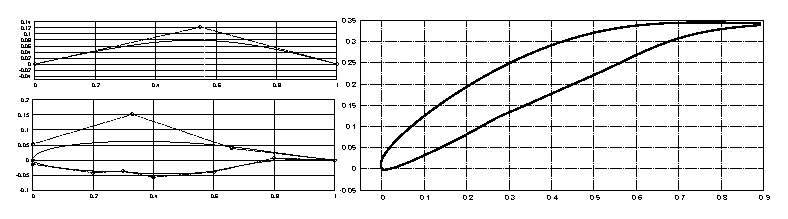
\includegraphics{blade_a.eps}}
\end{minipage}
\caption{Design of a compressor cascade using KBD: Archived design $B_1$.} 
\label{CBR_a}
\end{figure}

\begin{figure}[h!]
\begin{minipage}[b]{1\linewidth}
 \centering
 \resizebox*{15cm}{!}{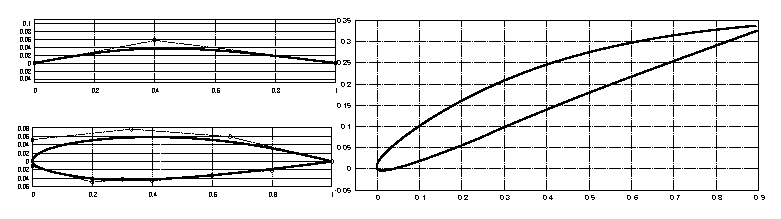
\includegraphics{blade_b.eps}}
\end{minipage}
\caption{Design of a compressor cascade using KBD: Archived design $B_2$.} 
\label{CBR_b}
\end{figure}

\begin{figure}[h!]
\begin{minipage}[b]{1\linewidth}
 \centering
 \resizebox*{15cm}{!}{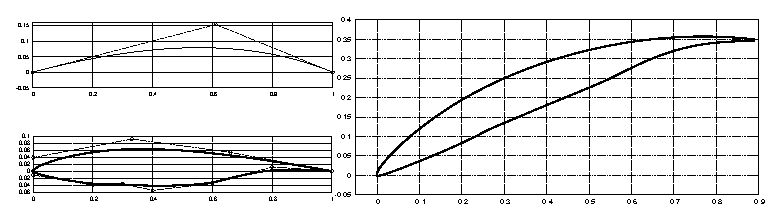
\includegraphics{blade_c.eps}}
\end{minipage}
\caption{Design of a compressor cascade using KBD: Archived design $B_3$.} 
\label{CBR_c}
\end{figure}

\begin{figure}[h!]
\begin{minipage}[b]{1\linewidth}
 \centering
 \resizebox*{15cm}{!}{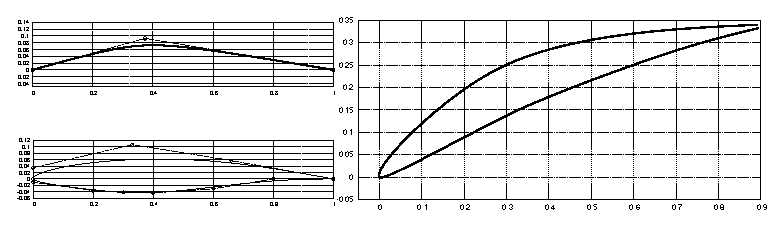
\includegraphics{blade_d.eps}}
\end{minipage}
\caption{Design of a compressor cascade using KBD: Archived design $B_4$.} 
\label{CBR_d}
\end{figure}



\begin{figure}[h!]
\begin{minipage}[b]{1\linewidth}
 \centering
 \resizebox*{15cm}{!}{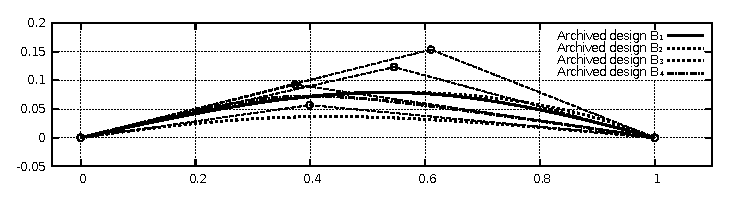
\includegraphics{mean_s.eps}}
\end{minipage}
\caption{Design of a compressor cascade using KBD: Mean-camber lines of the four bases. The observed great variance recommends the use of very extended design variable ranges during the EA-based optimization. This significantly deteriorates EA efficiency and makes the use of metamodels questionable. } 
\label{CBRDmm}
\end{figure}

\begin{figure}[h!]
\begin{minipage}[b]{1\linewidth}
 \centering
 \resizebox*{15cm}{!}{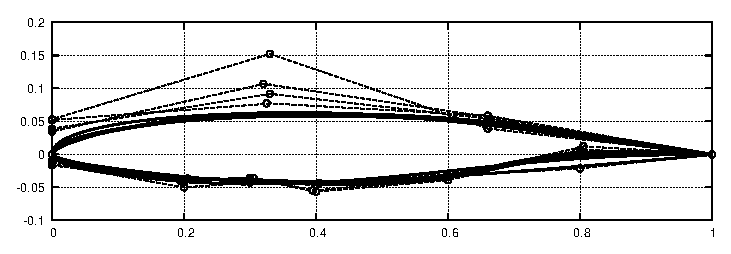
\includegraphics{thickness_s.eps}}
\end{minipage}
\caption{Design of a compressor cascade using KBD: Suction and pressure side thickness distributions and control point polygons for the four bases.} 
\label{CBRDtt}
\end{figure}


Four different optimization runs were performed in order to assess the effect of the KBD method both on EAs and the implementation of metamodels in MAEAs. The corresponding convergence plots are shown in fig.\ \ref{CBRDrela}. The use of metamodels in runs which do not rely upon the KBD method are not as efficient as expected. This is a caused by the use of an extended design space which is really necessary for being able to reproduce all four archived geometries. To demonstrate this, the four archived geometries are plotted together in figs.\ \ref{CBRDmm} and \ref{CBRDtt}. The large variance of the control points is more severe in the parameterization of the mean camber line (fig.\ \ref{CBRDmm}) regarding both coordinates and, also, in the thickness distribution along the suction side (fig.\ \ref{CBRDtt}). Using a more restricted design space would improve both the EA efficiency and the gain expected from the use of metamodels (MAEA) but could give suboptimal solutions if, by chance, the optimal geometry lays outside the design space. The comparison between EA and KBD-EA reveals the advantages of the proposed method (fig.\ \ref{CBRDrela}), since faster convergence is achieved. The comparison of KBD-MAEA with KBD-EA shows that the KBD method enhances the performance of the metamodel-based pre-evaluation phase. 

\begin{figure}[h!]
\begin{minipage}[b]{1\linewidth}
 \centering
 \resizebox*{12cm}{!}{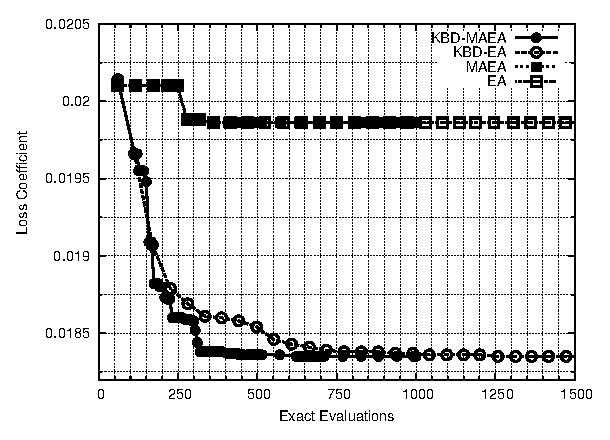
\includegraphics{Comp.eps}}
\end{minipage}
\caption{Design of a compressor cascade using KBD: Convergence comparison of four optimization runs using EA, KBD-EA, MAEA and KBD-MAEA. EA and MAEA have similar convergence plots, since the use of metamodels doesn't lead to extra gain, due to the extended range of the design variables. KBD-EA is significantly faster than  both EA and MAEA, thus proving the advantages of the proposed method. KBD-MAEA performs even better thanks to the positive effect of the proposed method on the use of metamodels.} 
\label{CBRDrela}
\end{figure}

The optimal blade resulting from the KBD-MAEA is presented in fig.\ \ref{CBRDrelaRes}. This design delivers $\omega\!=\!0.01834$ and $\Delta a\!=\!30.2^o$ at the desired flow conditions, outperforms any of the design-bases for the same flow-conditions and respects all the constraints. The airfoil designed using the KBD-MAEA is of significantly better quality compared with those delivered by the conventional runs, with or without the use of metamodels. 

\begin{figure}[h!]
\begin{minipage}[b]{1\linewidth}
 \centering
 \resizebox*{15cm}{!}{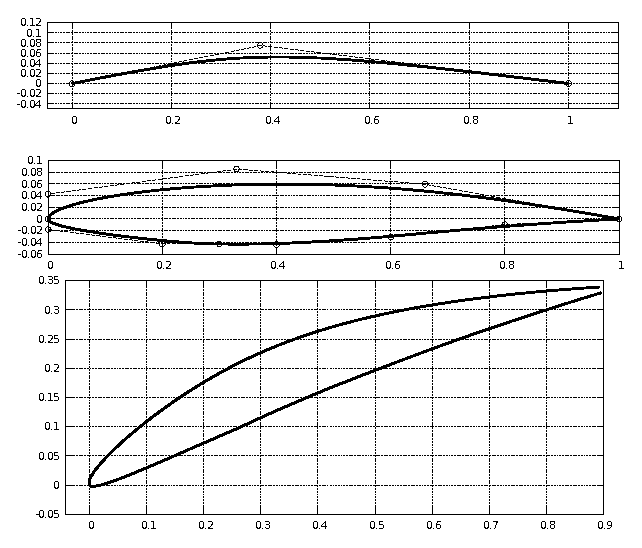
\includegraphics{ResD1.eps}}
\end{minipage}
\caption{Design of a compressor cascade using KBD: The optimal airfoil resulting from KBD-MAEA. Top: mean-camber line and thickness distributions together with their control polygons. Bottom: The airfoil shape after superimposing the thickness distribution on the mean-camber line and rotated at the desired stagger angle.} 
\label{CBRDrelaRes}
\end{figure}

%\begin{figure}[h!]
%\begin{minipage}[b]{1\linewidth}
% \centering
% \resizebox*{12cm}{!}{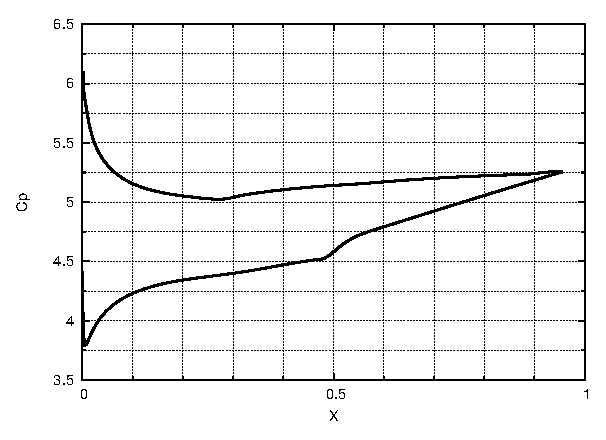
\includegraphics{Best_CP.eps}}
%\end{minipage}
%\caption{Pressure coefficient $C_p$ of the optimal airfoil fig.5\ref{CBRDrelaRes}.} 
%\label{CBRDrelaRes_cp}
%\end{figure}


%
% ---------------------------------------------------------------------------
% ----------------------- end of thesis sub-document ------------------------
% ---------------------------------------------------------------------------
